\section{Experimental Setup}
\label{sec:method}

We evaluate whether privileged-context on-policy self-distillation preserves the
test-time search behavior of thinking models. We write the on-policy
distillation objective in a context-explicit form, since our experiments vary
precisely what additional information the teacher receives. Given an input
problem $x$, the student policy $\pi_S$ samples an on-policy rollout
$y \sim \pi_S(\cdot \mid x)$. We then train the student by minimizing a
token-level divergence between the teacher and student next-token distributions
along this sampled rollout:
\[
\mathcal{L}_{\mathrm{OPD}}
=
\sum_t
D\left(
\pi_T(\cdot \mid x, c, y_{<t}),
\pi_S(\cdot \mid x, y_{<t})
\right).
\]
Here $y_{<t}$ is the prefix before token $t$, $\pi_T$ is the teacher policy,
$\pi_S$ is the student policy being updated, and $c$ denotes teacher-only
privileged context. The divergence $D$ can be instantiated as forward KL,
reverse KL, JSD, or another token-level distillation divergence. Vanilla OPD
corresponds to $c=\emptyset$, while privileged-context OPD sets $c$ to
additional information such as a final answer or gold demonstration. In
\opsd{}, the teacher and student share the same architecture and typically start
from the same checkpoint; in our experiments, the teacher is initialized as a
copy of the initial student checkpoint and receives privileged context while the
student does not. Unless otherwise noted, training rollouts are capped at
4,096 completion tokens. We use JSD distillation for one epoch with effective
batch size 64; this training cap is shared by the vanilla OPD, privileged OPD,
and \opsd{} comparisons. Full hyperparameter details are in
Appendix~\ref{app:experimental-details}.

\paragraph{Training data.}
We use two training domains. For math reasoning, we train on an OpenThoughts
15k subset, using the problem as the student prompt and the full reference
solution as the privileged teacher context. For Countdown, we train on 15k
examples from \texttt{jasonrqh/Countdown-CoT-20k}; the privileged context is the
post-thinking solution suffix. The Countdown split also reserves 500 held-out
examples for in-domain evaluation.

\paragraph{Models and comparisons.}
Our main comparisons separate instruct models from thinking models. On
Countdown, we train paired instruct and thinking models from the Qwen3-4B
\citep{yang2025qwen3} and OLMo-3-7B \citep{olmo2025olmo3} families to test
whether \opsd{} behaves differently when the base model already performs
explicit deliberation. On OpenThoughts, we focus on thinking models across
sizes and families, including \qwenonesevenb{},
\qwenfourb{}, \qweneightb{}, \qwenfourbthink{}, and \olmosevenbthink{}. We also
include controls that compare \opsd{} to vanilla OPD and that disable thinking
during \opsd{} training while keeping thinking enabled at evaluation.

\paragraph{Evaluation.}
We evaluate transfer to AIME 2024, AIME 2025, and HMMT 2025, and evaluate
Countdown-trained models on the held-out Countdown split. For AIME/HMMT, each
benchmark has 30 problems. To reflect standard evaluation practice for thinking
models, which often uses long rollout budgets to benefit from test-time compute
scaling, our main evaluation adopts a long generation cap: we generate 16
samples per problem, each with a maximum length of 38,912 tokens. This
evaluation cap is much larger than the default 4,096-token training completion
cap. Main tables report avg@16 accuracy, the mean sample correctness over the
16 rollouts for each problem.
Note that avg@16 is distinct from unbiased
pass@16, which measures whether at least one of the 16 samples solves the
problem. To compare the main long-budget setting with shorter evaluation settings, we repeat evaluation at generation caps of 4,096, 8,192, 16,384, 32,768, and 38,912 tokens, and also report pass@1\footnote{Empirical pass@1 is the same per-sample correctness quantity as avg@16, estimated from sampled rollouts under the evaluation decoding distribution.} and unbiased pass@16.

\section{Results}
\label{sec:results}

\subsection{\opsd{} helps instruct models but can degrade thinking models}

\begin{table*}[t]
\centering
\caption{\textbf{\opsd{} degrades thinking models across model families.}
We train each thinking model with privileged OpenThoughts solution context and evaluate on AIME24, AIME25, and HMMT25. Entries report avg@16 accuracy, and the Average column averages the three benchmarks. \opsd{} lowers the average score for all five thinking models, suggesting that the degradation is not specific to one model size or family.}
\label{tab:openthoughts_thinking_models}
\small
\setlength{\tabcolsep}{5pt}
\renewcommand{\arraystretch}{1.15}

\newcommand{\metrichead}[1]{%
  \textbf{#1}%
}

\begin{tabular*}{\textwidth}{@{\extracolsep{\fill}}llcccc@{}}
\toprule
\textbf{Model}
&
& \metrichead{AIME24}
& \metrichead{AIME25}
& \metrichead{HMMT25}
& \metrichead{Average} \\
\midrule

\multirow{2}{*}{\textbf{\qwenonesevenb{} (Thinking)}}
& \textbf{Base}
& \textbf{0.502}
& \textbf{0.398}
& \textbf{0.215}
& \textbf{0.372} \\
&
\textbf{+\opsd{}}
& 0.435
& 0.302
& 0.185
& 0.308 \\
\midrule

\multirow{2}{*}{\textbf{\qwenfourb{} (Thinking)}}
& \textbf{Base}
& \textbf{0.727}
& \textbf{0.635}
& \textbf{0.410}
& \textbf{0.591} \\
&
\textbf{+\opsd{}}
& 0.683
& 0.556
& 0.362
& 0.534 \\
\midrule

\multirow{2}{*}{\textbf{\qweneightb{} (Thinking)}}
& \textbf{Base}
& \textbf{0.758}
& \textbf{0.700}
& \textbf{0.448}
& \textbf{0.635} \\
&
\textbf{+\opsd{}}
& 0.721
& 0.613
& 0.400
& 0.578 \\
\midrule

\multirow{2}{*}{\textbf{\qwenfourbthink{}}}
& \textbf{Base}
& \textbf{0.804}
& \textbf{0.804}
& \textbf{0.552}
& \textbf{0.720} \\
&
\textbf{+\opsd{}}
& 0.787
& 0.731
& 0.529
& 0.683 \\
\midrule

\multirow{2}{*}{\textbf{\olmosevenbthink{}}}
& \textbf{Base}
& \textbf{0.719}
& \textbf{0.667}
& \textbf{0.452}
& \textbf{0.612} \\
&
\textbf{+\opsd{}}
& 0.715
& 0.652
& 0.446
& 0.604 \\

\bottomrule
\end{tabular*}
\end{table*}


\begin{table*}[t]
\centering
\caption{\textbf{\opsd{} helps instruct models more reliably than thinking models on Countdown.}
We use \opsd{} to train various models on Countdown and evaluate on held-out Countdown data, AIME24, AIME25, and HMMT25. Entries report avg@16 accuracy, and the Average column averages the four benchmarks. Instruct Qwen and OLMo models improve under \opsd{}, while the corresponding thinking models show smaller or mixed gains.}
\label{tab:countdown_think_vs_instruct}
\small
\setlength{\tabcolsep}{5pt}
\renewcommand{\arraystretch}{1.15}

\newcommand{\metrichead}[1]{%
  \textbf{#1}%
}

\begin{tabular}{@{}llccccc@{}}
\toprule
\textbf{Model} &
& \metrichead{Countdown}
& \metrichead{AIME24}
& \metrichead{AIME25}
& \metrichead{HMMT25}
& \metrichead{Average} \\
\midrule

\multirow{2}{*}{\textbf{\qwenfourbinstruct{}}}
& \textbf{Base}
& 0.736
& \textbf{0.604}
& 0.463
& \textbf{0.304}
& 0.527 \\
&
\textbf{+\opsd{}}
& \textbf{0.865}
& 0.594
& \textbf{0.483}
& 0.294
& \textbf{0.559} \\
\midrule

\multirow{2}{*}{\textbf{\qwenfourbthink{}}}
& \textbf{Base}
& 0.945
& \textbf{0.804}
& \textbf{0.804}
& \textbf{0.552}
& \textbf{0.776} \\
&
\textbf{+\opsd{}}
& \textbf{0.947}
& 0.800
& 0.775
& 0.537
& 0.765 \\
\midrule

\multirow{2}{*}{\textbf{\olmosevenbinstruct{}}}
& \textbf{Base}
& 0.719
& \textbf{0.525}
& \textbf{0.415}
& 0.237
& 0.474 \\
&
\textbf{+\opsd{}}
& \textbf{0.814}
& 0.510
& 0.394
& \textbf{0.256}
& \textbf{0.494} \\
\midrule

\multirow{2}{*}{\textbf{\olmosevenbthink{}}}
& \textbf{Base}
& 0.877
& 0.719
& 0.667
& \textbf{0.452}
& 0.679 \\
&
\textbf{+\opsd{}}
& \textbf{0.890}
& \textbf{0.742}
& \textbf{0.698}
& \textbf{0.452}
& \textbf{0.695} \\

\bottomrule
\end{tabular}
\end{table*}


\begin{table}[t]
\centering
\caption{\textbf{The degradation depends on whether thinking is enabled during \opsd{} training.}
We train on OpenThoughts 30k and evaluate with thinking mode in all rows. When thinking is enabled during \opsd{} training, \qwenfourb{} loses avg@16 accuracy on all three math evaluations; disabling thinking during training preserves the base-model average while still evaluating with thinking enabled.}
\label{tab:openthoughts_thinking_enabled_disabled}
\small
\setlength{\tabcolsep}{8pt}
\renewcommand{\arraystretch}{1.15}
\begin{tabular*}{\linewidth}{@{\extracolsep{\fill}}lcccc@{}}
\toprule
\textbf{Method}
& \textbf{AIME24}
& \textbf{AIME25}
& \textbf{HMMT25}
& \textbf{Avg.} \\
\midrule
\qwenfourb{}
& 0.727
& 0.635
& 0.410
& 0.591 \\
+\opsd{} (Thinking)
& 0.667
& 0.571
& 0.358
& 0.532 \\
+\opsd{} (No Thinking)
& 0.731
& 0.615
& 0.423
& 0.590 \\
\bottomrule
\end{tabular*}
\end{table}


\opsd{} training helps instruct models more reliably than
thinking models. In the Countdown-trained setting
(Table~\ref{tab:countdown_think_vs_instruct}), \qwenfourbinstruct{} and
\olmosevenbinstruct{} improve under \opsd{} ($0.527 \to 0.559$ and
$0.474 \to 0.494$ avg@16 performance). The matched thinking models show mixed
results: \qwenfourbthink{} drops slightly ($0.776 \to 0.765$), while
\olmosevenbthink{} gains modestly ($0.679 \to 0.695$).
Appendix~\ref{app:sd-zero-srt} shows a similar pattern in an SD-Zero-style
self-revision pipeline \citep{he2026selfdistillationzero}: the self-revision
stage helps both the instruction-tuned and thinking models, but the subsequent
\opsd{} stage further helps only the instruction-tuned model and hurts the
thinking model.

Thinking model degradation is clearest in the OpenThoughts-trained setting
(Table~\ref{tab:openthoughts_thinking_models}). Across model scale and family,
all five thinking models we evaluate lose avg@16 performance under the same
training recipe, with drops ranging from $6.4$ points (\qwenonesevenb{}) to
$0.8$ points (\olmosevenbthink{}).
Paired problem-level bootstrap intervals for the main average deltas are
reported in Appendix~\ref{app:bootstrap-cis}; in this setting, the intervals
exclude zero for four of the five comparisons, including all Qwen variants.

For thinking models, \opsd{} degrades performance when the rollouts being supervised are thinking rollouts.
Table~\ref{tab:openthoughts_thinking_enabled_disabled} holds
the model fixed (\qwenfourb{}) and evaluates with thinking enabled in all rows.
When training rollouts are non-thinking, performance is preserved ($0.591 \to 0.590$); when they are thinking, performance drops to $0.532$.

\subsection{Thinking-model degradation is specific to teacher-side privileged context}

\begin{table*}[t]
\centering
\caption{\textbf{Privileged teacher context, not on-policy distillation itself, degrades thinking-model performance.}
On a \qwenonesevenb{} thinking student, vanilla OPD with a larger \qweneightb{} teacher improves avg@16 accuracy over the base model. However, conditioning the teacher on information unavailable to the student at test time makes the resulting on-policy update harmful on average. This occurs both for a larger teacher (OPD gold demo) and for the self-teacher (OPSD) setting. All OPD/OPSD variants are trained with a 4,096-token completion cap; all methods, including the base model, are evaluated with a 38,912-token generation cap.}
\label{tab:qwen17_openthoughts_opsd_opd}
\footnotesize
\setlength{\tabcolsep}{3pt}
\renewcommand{\arraystretch}{1.12}

\newcommand{\metrichead}[1]{%
  \textbf{#1}%
}

\begin{tabular*}{\textwidth}{@{\extracolsep{\fill}}llcccc@{}}
\toprule
\textbf{Model}
&
& \metrichead{AIME24}
& \metrichead{AIME25}
& \metrichead{HMMT25}
& \metrichead{Average} \\
\midrule

\multirow{4}{*}{\textbf{\qwenonesevenb{}}}
& \textbf{Base}
& 0.502
& \textbf{0.398}
& 0.215
& 0.372 \\

&
\textbf{+\opsd{}}
& 0.435
& 0.302
& 0.185
& 0.308 \\

&
\textbf{+OPD}
& \textbf{0.540}
& 0.385
& \textbf{0.252}
& \textbf{0.392} \\

&
\textbf{+OPD gold demo}
& 0.467
& 0.344
& 0.240
& 0.350 \\

\bottomrule
\end{tabular*}
\end{table*}


The same student improves under vanilla on-policy distillation, where the teacher is
not given privileged context. In
Table~\ref{tab:qwen17_openthoughts_opsd_opd}, vanilla OPD trains
\qwenonesevenb{} against a larger teacher that sees the same prompt, improving
avg@16 performance from $0.372$ to $0.392$. Adding privileged context reverses
the sign: context-enhanced OPD with a privileged gold demonstration reduces
performance to $0.350$, and \opsd{} with a full gold demonstration reduces it
to $0.308$. Performance falls when
the teacher scores the student's trajectory while conditioned on information the
student will not have at test time.

\subsection{The degradation appears when models are allowed to think longer}

\begin{figure}[t]
    \centering
    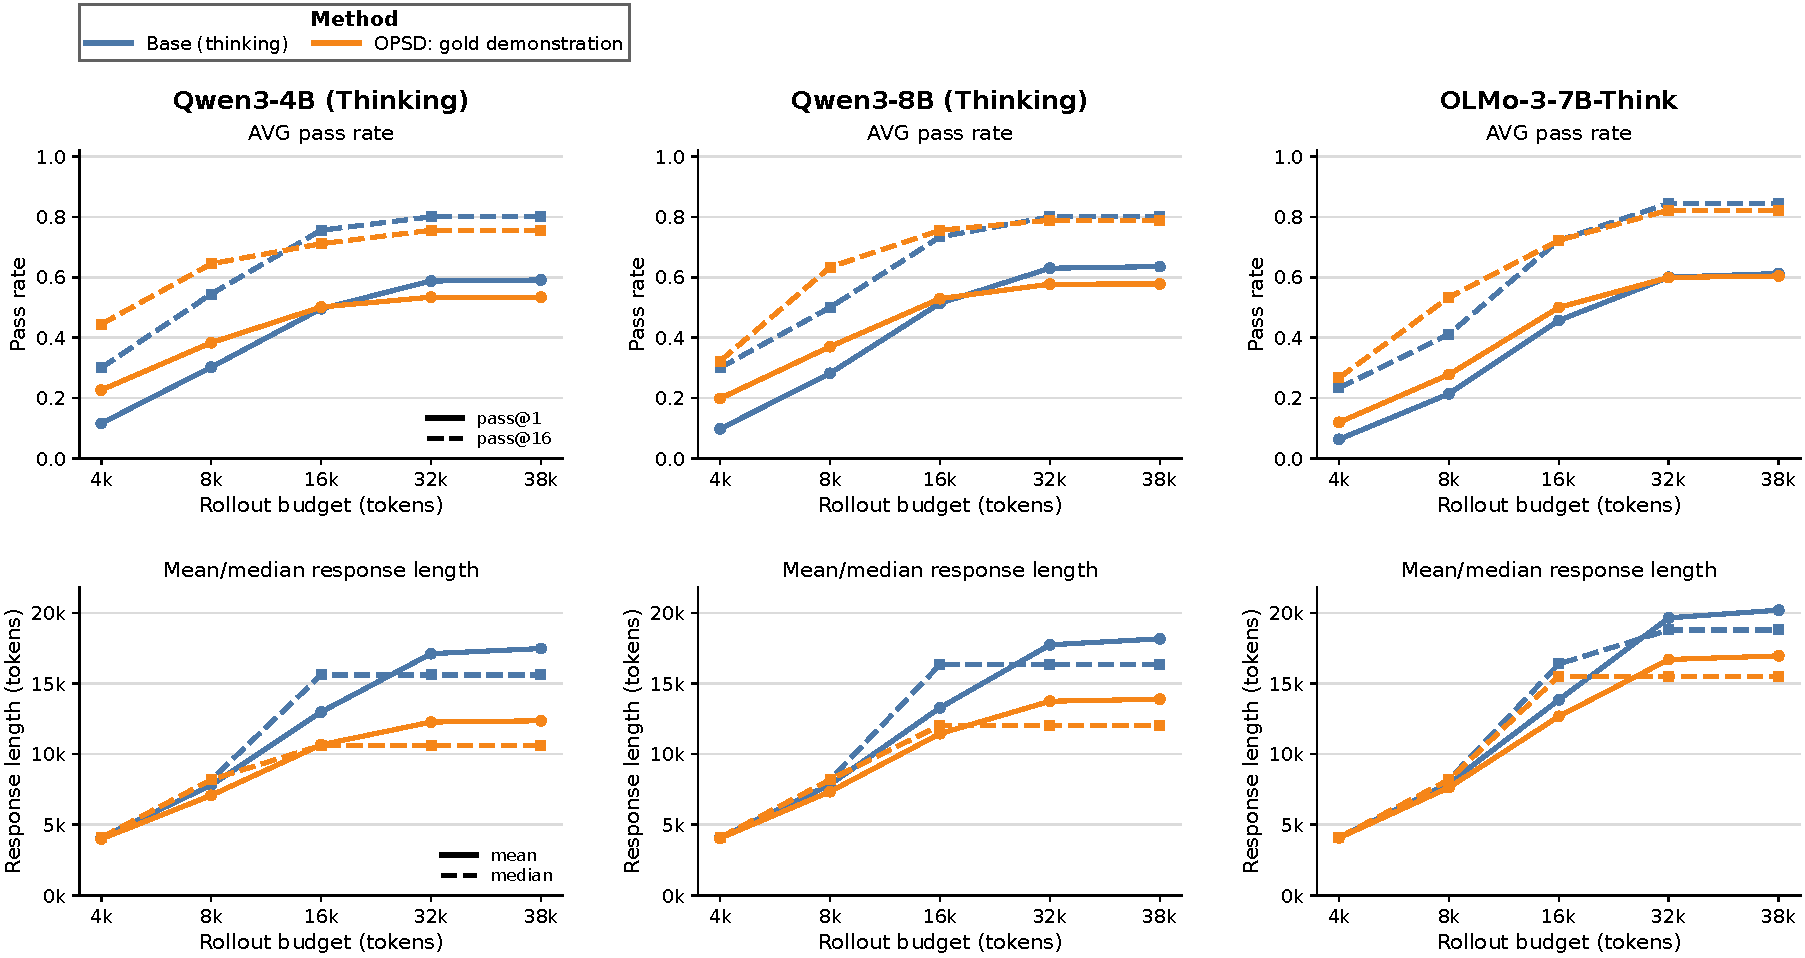
\includegraphics[width=\linewidth]{figures/avg_pass_and_rollout_tokens_qwen_olmo_demo_only.pdf}
    \caption{
    \textbf{For thinking models, \opsd{} can improve short-budget performance via compression but can hurt long-budget reasoning.}
    We evaluate OpenThoughts-trained Qwen3-4B, Qwen3-8B, and OLMo-3-7B thinking models across rollout budgets. Models are trained with a 4,096-token completion cap and evaluated at generation caps from 4,096 to 38,912 tokens. Top row: pass@1 and pass@16, averaged over AIME24, AIME25, and HMMT25. Bottom row: mean and median response length. \opsd{} with gold demonstrations often helps at 4k--8k tokens, but the advantage shrinks or reverses at 32k--38k tokens, where responses become substantially shorter than the base model.
    }
    \label{fig:openthoughts_accuracy_length_collapse}
\end{figure}


The degradation in thinking-model performance is concentrated at long rollout
budgets.
Figure~\ref{fig:openthoughts_accuracy_length_collapse} evaluates
OpenThoughts-trained \qwenfourb{}, \qweneightb{}, and \olmosevenbthink{} across
rollout budgets from 4k to 38k tokens. At 4k--8k tokens, \opsd{} models perform
comparably to or above their bases\footnote{Throughout this section, ``base''
denotes the corresponding instruct or thinking checkpoint before additional
\opsd{}/OPD training, not a pretrained base model.}. By 32k--38k tokens, they match or fall
below. Response length follows the same pattern: at small budgets, base and
\opsd{} rollouts are similar in length; at large budgets, \opsd{} rollouts are
substantially shorter. Overall, \opsd{} removes the gains that thinking models obtain from longer rollouts.

One might suspect a simpler explanation based on the mismatch between training
and evaluation lengths. Training rollouts are capped at 4,096 tokens, whereas
evaluation allows much longer rollouts, so short-budget training may cause the
model to forget longer reasoning behaviors. The OPD experiments rule out this
explanation as the sole cause. In
Table~\ref{tab:qwen17_openthoughts_opsd_opd}, vanilla OPD with a larger
unprivileged teacher improves the student under the same short-budget on-policy
setup, whereas adding teacher-only gold-demonstration context reverses the gain.
The corresponding budget curves in
Figure~\ref{fig:qwen17_opd_gold_demo_budget_curves} show that the two OPD
variants differ not only in accuracy but also in realized response length:
vanilla OPD largely preserves the base response-length behavior, while
gold-demonstration OPD shortens responses and reduces the pass@1 gains. Thus,
the drop cannot be attributed only to the train/eval budget mismatch; it also
depends on whether the teacher scores the short-budget rollout with privileged
context.

\subsection{Students inherit shorter rollouts but not the teacher's pass@k gains}

\begin{figure}[t]
    \centering
    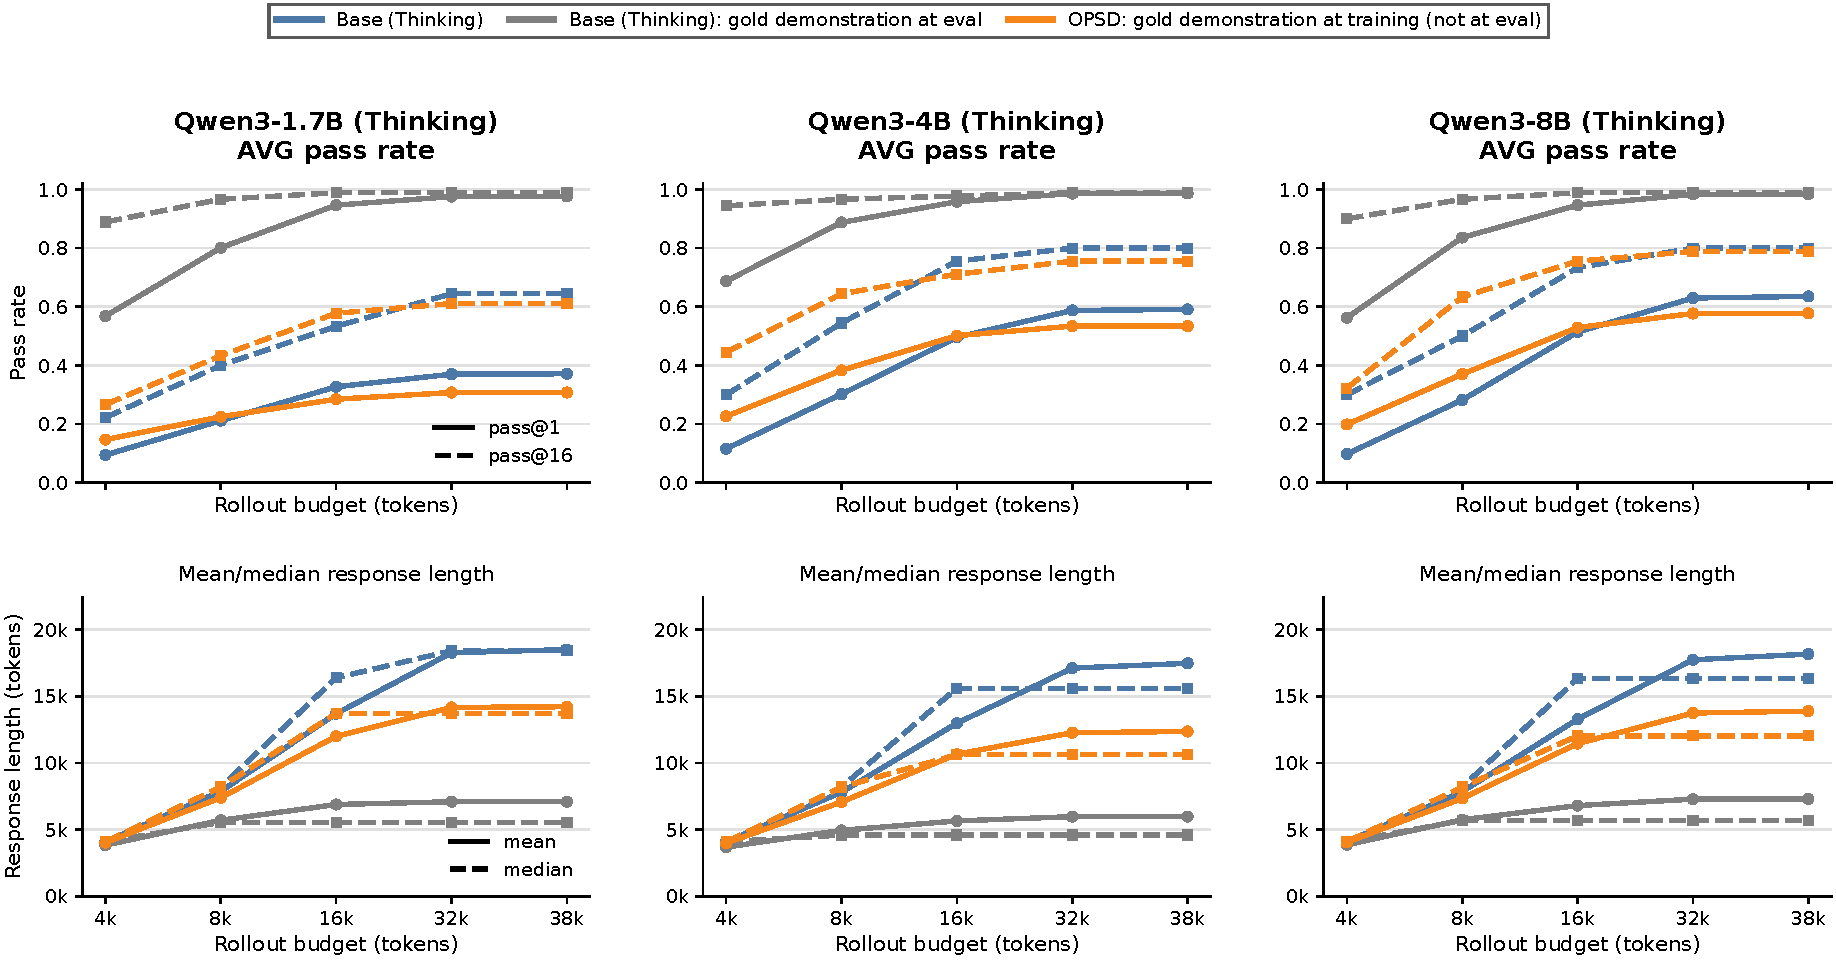
\includegraphics[width=\linewidth]{figures/avg_pass_rollout_tokens_qwen_gpt_oss_final_response_with_opsd_demo_purple_context.pdf}
    \caption{
    \textbf{\opsd{} students inherit the teacher's shorter response lengths, but not the pass@k benefits at longer rollout budgets.}
    For each Qwen3 thinking-model size (1.7B, 4B, and 8B), we compare three settings: the base model; the same base model given a gold demonstration in context, matching the setup of the \opsd{} teacher; and the \opsd{} student, evaluated without the gold demonstration in context.
    Top row: pass@1 and pass@16, averaged over AIME24, AIME25, and HMMT25.
    Bottom row: mean and median response length.
    Providing the teacher with the gold demonstration in context shortens the teacher's own rollouts without hurting pass@k, and can even improve pass@k.
    Though the \opsd{} student produces shorter responses like the teacher, the student's pass@k gains are smaller at short budgets and disappear or reverse at longer rollout budgets.
    }
    \label{fig:openthoughts_teacher_student_asymmetry}
\end{figure}


We next evaluate whether the gold-demo-conditioned base model---the \opsd{}
teacher setup---exhibits the long-budget degradation observed in the \opsd{}
student. Figure~\ref{fig:openthoughts_teacher_student_asymmetry} compares three
settings for each Qwen3 thinking-model size: the base model without privileged
context, the \opsd{} teacher (the base model when provided the in-context gold
demonstration), and the \opsd{}-trained student evaluated without the in-context
gold demonstration. The teacher's own rollouts become much shorter, but its
pass@k remains high and often improves. The student also produces shorter
responses, but compared with the teacher's gains over
the unprivileged base, the student's pass@k gains are smaller at short budgets
and disappear or reverse at longer budgets. Thus, the student inherits the
teacher's shorter response behavior more reliably than the teacher's
privileged-context performance benefits.

\subsection{Sparse privileged context preserves long-budget behavior better than dense privileged context}

\begin{figure}[t]
    \centering
    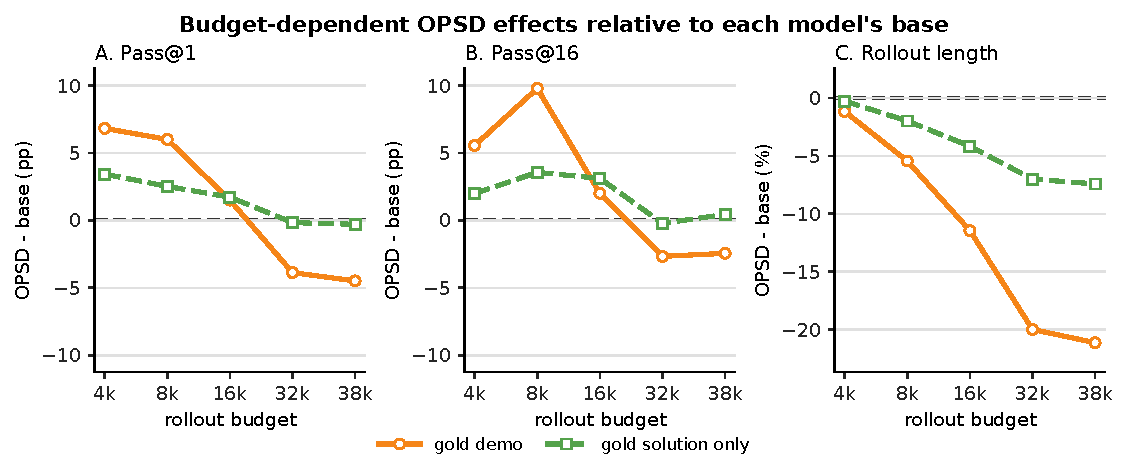
\includegraphics[width=\linewidth]{figures/openthoughts_privinfo_budget_crossover.pdf}
    \caption{
    \textbf{In thinking models, sparse privileged context preserves long-budget behavior better than dense demonstrations.}
    We plot \opsd{} minus each model's base performance across rollout budgets, averaged over the thinking models in Table~\ref{tab:openthoughts_thinking_models}. Panels A and B show pass@1 and pass@16 changes in percentage points; Panel C shows relative rollout-length change. Dense gold demonstrations give larger short-budget gains but turn negative at long budgets and strongly shorten responses, while the sparse gold-solution hint remains closer to the base model.
    }
    \label{fig:openthoughts_sparse_context}
\end{figure}


We next ask whether the student-side degradation depends on how much privileged
context the teacher receives, and observe that full gold demonstrations degrade
long-budget behavior more than final-answer-only context.
Figure~\ref{fig:openthoughts_sparse_context} compares these two forms
of privileged context, averaged over the models in
Table~\ref{tab:openthoughts_thinking_models}. Full demonstrations give the
largest short-budget gains in pass@1 and pass@16, but also the largest
long-budget reversals, with mean rollout length compressed to roughly
$0.8\times$ the base at 38k tokens. The final-answer-only condition gives
smaller short-budget gains, remains closer to the base at long budgets, and
produces less length compression. Because the answer-only and full-demonstration
runs use the same training recipe and 4,096-token completion cap, this difference
cannot be explained by the short training budget alone; it depends on how much
privileged context the teacher receives.

In Section~\ref{sec:analysis}, we show that \opsd{} reduces fork rates at
high-entropy decision points and reduces explicit deliberation markers in
evaluation rollouts.
